\documentclass[../main.tex]{subfiles}
\begin{document}

\section{Motivation}

\subsection{Anforderungen}


Die Entwicklung des hier beschriebenen Schreibassistenten verfolgt das Ziel, ein innovatives \glslink{glos:ki}{KI}-Werkzeug zu schaffen, das vor allem Schüler und Studenten bei dem Verfassen 
verschiedener Texte unterstützt. Die von Studenten genutzten Text-Editoren wie Overleaf sollen nicht ersetzt werden. Stattdessen soll eine Möglichkeit geboten werden, 
\glslink{glos:ki}{KI}-Chats mit unterschiedlichen \glslink{glos:llm}{LLM}s übersichtlich zu sammeln. Es soll, wie in \autoref{sec:nachteile} beschrieben, eine Art "`\glslink{augmented-intelligence}{Augmented Intelligence}"' geschaffen werden, die die Effizienz im Schreibprozess 
steigert, aber nicht das komplette Verfassen übernimmt.\\ Im Gegensatz zu den in \autoref{sec:bereitsBestehendeLoesungen} beschriebenen bestehenden Lösungen, sollen verschiedene \glslink{glos:ki}{KI}-Chats 
übersichtlich und abschnittsbezogen angelegt werden können. Für jeden Textabschnitt können mehrere \glslink{glos:ki}{KI}-Chats mit unterschiedlichen Modellen erstellt und gespeichert werden. Durch das Sammeln 
der \glslink{glos:ki}{KI}-Chats soll ein übersichtlicheres Arbeiten ermöglicht werden. Zudem kann der Nutzer die \glslink{glos:ki}{KI}-Antworten kommentieren, um sich Gedanken zu Verbesserungen oder zu der Relevanz der generierten Antwort für den Text zu notieren.\\
Darüber hinaus soll es möglich sein, ein KI-Nutzungsverzeichnis zu generieren. So soll die Nutzung der KI transparent und nachvollziehbar dargestellt werden.\\
Das Nutzerinterface des Schreibassistenten soll intuitiv und verständlich gestaltet sein. Um unerfahrenen Nutzern den Umgang mit 
generativer \glslink{glos:ki}{KI} zu vereinfachen, werden die in \autoref{ch:anforderungen} identifizierten Anforderungen umgesetzt. Dazu gehören \glslink{tooltips}{Tooltips} an Knöpfen, die mit der 
\glslink{glos:ki}{KI}-Funktionalität verbunden sind. Diese erklären dem Nutzer die jeweilige Funktion. Jeder Nutzer soll nachvollziehen können, welchen Einfluss eine Eingabe in 
ein Textfeld oder eine Auswahl aus einem Drop-Down-Menü auf die Antwort hat. Zudem wird der Nutzer beim Anlegen eines Projekts gewarnt, dass 
\glslink{glos:ki}{KI}-Modelle halluzinieren können. Damit soll, ähnlich wie in der in \autoref{ch:anforderungen} behandelten Studie, die Akzeptanz von \glslink{glos:ki}{KI}-generierten Misinformationen verringert werden. Dadurch 
wird das Risiko, dass Fehlinformationen in Arbeiten von Schülern und Studenten gelangen, reduziert. Der Nutzer soll angeregt werden, die von der \glslink{glos:ki}{KI} generierten Inhalte 
\mbox{kritisch zu hinterfragen.}\\
Auch bei der Formulierung von \gls{glos:prompt}s soll der Nutzer Unterstützung erhalten. Da bereits kleine Änderungen im Prompt oder in der Reihenfolge der Informationen großen 
Einfluss auf die \glslink{glos:ki}{KI}-Antwort haben können, sind verlässliche und reproduzierbare Abläufe schwer zu erreichen \cite{creativeWriting}. Dies soll durch das Zusammensetzen vorgefertigter 
Prompts im Backend umgangen werden. So wird die Nutzung für \glslink{glos:ki}{KI}-Unerfahrene erleichtert. Dafür werden Prompts für diese in \autoref{sec:vorteile} identifizierten 
Einsatzmöglichkeiten bereitgestellt: umformulieren, zusammenfassen, Text aus Stichpunkten erstellen, Synonyme finden, Grammatik und Rechtschreibung prüfen sowie Feedback geben. Außerdem soll das KI-Modell
Schülern Sachverhalte erklären können, um das Erarbeiten eines Themas effizienter zu gestalten.


\subsection{Anwendungsfälle}

Der Schreibassistent wird für unterschiedliche Anwendungsfälle entwickelt: 
 Zum einen soll dem Nutzer ein Werkzeug geboten werden, mit welchem er strukturiert verschiedene \glslink{glos:ki}{KI}-Modelle verwenden kann. Die bereitgestellten vorgefertigten \gls{glos:prompt}s sollen 
 die Effizienz während des Schreibprozesses weiter steigern. Darüber hinaus ist das Schreiben nutzerdefinierter Prompts möglich. Das generierte \glslink{glos:ki}{KI}-Nutzungsverzeichnis kann als eine 
 Art Quellenverzeichnis an wissenschaftliche Arbeiten angehangen werden. Es zeigt das verwendete \glslink{glos:ki}{KI}-Modell, die Aufgabe, welche das Modell übernehmen sollte 
 beziehungsweise den Prompt, sowie das Datum der Anfrage. In diesem Nutzungsverzeichnis werden nur Prompts zu den gespeicherten Chats angeführt. Dadurch wird vermieden, dass Chats 
 vermerkt werden, deren Ergebnisse nicht in die Arbeit eingeflossen sind, und das Verzeichnis bleibt übersichtlich.\\ 
 Der zweite Anwendungsfall ist der sogenannte Schülermodus. Durch 
 Einschränken der Funktionalität soll ein Werkzeug zur Verfügung gestellt werden, welches zu Unterrichtszwecken verwendet werden kann. Schüler sollen so den Umgang mit generativer 
 \glslink{glos:ki}{KI} erlernen, ohne den gesamten Text von dem \glslink{glos:ki}{KI}-Modell schreiben zu lassen. Die entstandenen Texte sind Eigenleistung des Schülers, jedoch kann der 
 Schreibprozess durch den KI-Einsatz effizienter gestaltet werden, was die in \autoref{sec:vorteile} beschriebenen Vorteile mit sich bringt. Der Schüler kann aus den vorgefertigten Aufgaben 
 wählen, jedoch keinen eigenen Prompt verwenden. Dadurch soll verhindert werden, dass ganze Texte \glslink{glos:ki}{KI}-generiert werden. Zudem wird, anders als im normalen Modus, jeder 
 Chat im \glslink{glos:ki}{KI}-Nutzungsverzeichnis vermerkt. Dies sorgt für bessere Nachvollziehbarkeit des \glslink{glos:ki}{KI}-Einsatzes für Lehrkräfte.\\ 
 Zuletzt soll der Schreibassistent 
 beim Schreiben von benoteten Arbeiten während des Unterrichts eingesetzt werden können. Dazu dient der Prüfungsmodus. Es kann eine bestimmte Bearbeitungszeit eingestellt werden. 
 Ist diese abgelaufen, wird der entstandene Text automatisch abgegeben. Das \glslink{glos:ki}{KI}-Nutzungsverzeichnis wird wie im Schülermodus erstellt, sodass alle \glslink{glos:ki}{KI}-Chats 
 erkennbar sind. Überdies  wird das Öffnen anderer Projekte oder Tabs verhindert. Sollte ein Schüler versuchen, andere \glslink{glos:ki}{KI}-Werkzeuge oder Hilfsmittel zu verwenden, 
 wird die Arbeit automatisch abgegeben. Dadurch soll sichergestellt werden, dass das Schreiben der Arbeit weiterhin eine Eigenleistung des Schülers ist. Die \glslink{glos:ki}{KI} hilft 
 bei der Formulierung und Rechtschreibung des Textes, den Inhalt muss jedoch der Schüler verfassen. Insgesamt soll eine sichere Umgebung zur Verfügung gestellt werden, wodurch der Einsatz 
 generativer \glslink{glos:ki}{KI} während des Unterrichts ermöglicht wird.


\section{Verwendete Technologien}

Das Frontend des Schreibassistenten wurde mit dem Framework React entwickelt. Diese JavaScript-Bibliothek verfolgt einen komponentenbasierten Ansatz, welcher die Mehrfachnutzung 
von Codeteilen gestattet. React TypeScript bietet zusätzlich Typisierung, wodurch der Code weniger fehleranfällig ist. React wurde primär wegen seiner Performanz und Dynamik gewählt. \cite{react1,react2} \\
Für das Design kommt Cascading Style Sheets (CSS) zum Einsatz. Die Nutzung eigener \acrshort{css}-Klassen erlaubt Wiederverwendbarkeit. Im Gegensatz zu CSS-Frameworks ermöglicht reines CSS größere Flexibilität.\\
Das Backend ist mit dem Web-Framework FastAPI umgesetzt. Dieses Python-Framework zeichnet sich durch gute Performanz und eingebaute Typisierung aus. Die Verwendung von Datenmodellen verbessert die Code-Qualität \cite{fastapi}.\\
Python als Programmiersprache erleichtert die Umsetzung, da sie einfach aufgebaut und weit verbreitet ist. Zudem existieren zahlreiche \mbox{zusätzliche Bibliotheken. \cite{python}}\\
Eine dieser Bibliotheken ist SQLAlchemy, die für die Implementierung verwendet wurde. Sie bietet eine objektorientierte Abstraktionsschicht für den Datenbankzugriff, sodass mit Python-Klassen statt mit \acrshort{sql}-Abfragen gearbeitet werden kann. 
So wird der Code übersichtlicher und wartbarer. Der Zugriff auf die verwendete SQLite-Datenbank wird erleichtert. Ein Umstieg auf eine leistungsfähigere Datenbank wäre später mit wenig Aufwand möglich. \cite{SQLAlchemy}\\
Für die Einbindung der \glslink{glos:ki}{KI}-Modelle wurde \glslink{ollama}{Ollama} verwendet. Ollama ist eine \glslink{open-source}{Open-Source}-Software, die die Ausführung von \glslink{glos:llm}{LLM}s lokal ermöglicht. 
Sie stellt eine \acrshort{api1} zur Verfügung, über die verschiedene Modelle genutzt werden können. Ollama übernimmt den Wechsel zwischen Modellen, verhindert Parallelnutzung und erhöht so die Performanz. \cite{ollamaSchreibassi,ollamaTechnologie}



\section{Verwendete \glslink{glos:ki}{KI}-Modelle} \label{sec:kiModelle}

Mit Ollama können verschiedene \glslink{glos:ki}{KI}-Modelle lokal und damit datenschutzkonform genutzt werden. Somit werden die in \autoref{sec:datenschutz} beschrieben Nachteile umgangen. 
Nutzer können frei zwischen mehreren Modellen wählen und selbst festlegen, welche verfügbar sind. Für Einsteiger wird zu jeder Aufgabe ein empfohlenes Modell mit passendem, 
getestetem Prompt vorgeschlagen. Die getesteten Modelle sind auf gute Ergebnisse bei deutscher Sprache und Performanz auf aktuellen Laptops ausgelegt. Dabei erfolgten stichprobenartige 
Prüfungen der Antworten auf Ausdruck, Grammatik und Inhalt, um zu bestimmen, welches Modell standardmäßig für welche Aufgabe vorgeschlagen werden soll. Im Folgenden werden die wichtigsten \mbox{Testergebnisse beleuchtet:}

\begin{itemize} \item \textbf{lukasmalkmus/llama3-sauerkraut} (8 Mrd. \glslink{parameter}{Parameter}, auf Llama-3 basierend)\cite{sauerkraut}: Antwortet teils auf Englisch oder ersetzt deutsche Begriffe. Wird daher im Schreibassistenten nicht verwendet.

\item \textbf{mayflowergmbh/wiedervereinigung} (auf Mistral basierend, 7 Mrd. Parameter) \cite{wiedervereinigung}: Fügt oft neuen Inhalt hinzu statt der Aufgabe zu folgen. Nicht verwendet.

\item \textbf{mayflowergmbh/wiederchat} (7 Mrd. Parameter) \cite{wiederchat}: Führt Prompts oft nicht ganz aus, liefert aber beim Zusammenfassen die besten Stichpunkt-Antworten. Wird dafür empfohlen.

\item \textbf{jobautomation/OpenEuroLLM-German} (auf Gemma 3 basierend) \cite{openeurollm}: Generiert vollständige und gut strukturierte Texte, keine fremdsprachigen Fachwörter. Für das Erstellen eines Textes aus Stichpunkten und Umformulieren als Standard-Modell gewählt.

\item \textbf{Gemma3} (von Google entwickelt, Open Source, 12 Mrd. Parameter) \cite{gemma3}: Aufgrund fehlender Spezialisierung meist weniger gut formulierte Texte, aber sehr gut geeignet für Synonyme, Feedback, Überprüfung der Grammatik sowie erklären von Sachzusammenhängen. \end{itemize}

Die Einbindung der Modelle erfolgt über die lokale \glslink{ollama}{Ollama}-API. Für jeden \glslink{glos:ki}{KI}-Aufruf sendet das Backend die Modellwahl sowie Inhalte wie Aufgabe, bisherigen Chatverlauf, 
Paragraphinhalt, gegebenenfalls Nutzerkommentare und weitere Felder an Ollama.\\ Die Prompts für jede Aufgabe wurden getestet und iterativ angepasst, bis die Modelle zufriedenstellende Antworten 
lieferten. Sie sind auf Deutsch verfasst, da der Schreibassistent auf die deutsche Sprache spezialisiert ist. Englische Prompts führten im Test zu keinen signifikant besseren Ergebnissen. Die Ergebnisse des Prompt-Engineerings befinden sich in Anhang \ref{Prompts}.\\
Erstellt der Nutzer ein Projekt wird automatisch geprüft, ob die für die Standardaufgaben vorgeschlagenen KI-Modelle installiert sind. Sollte dies nicht der Fall sein, werden sie heruntergeladen.
Darüber hinaus kann der Nutzer den Schreibassistenten verwenden, um weitere KI-Modelle zu laden. 

\section{Aufbau der Datenbank}
\begin{figure}[h!]
  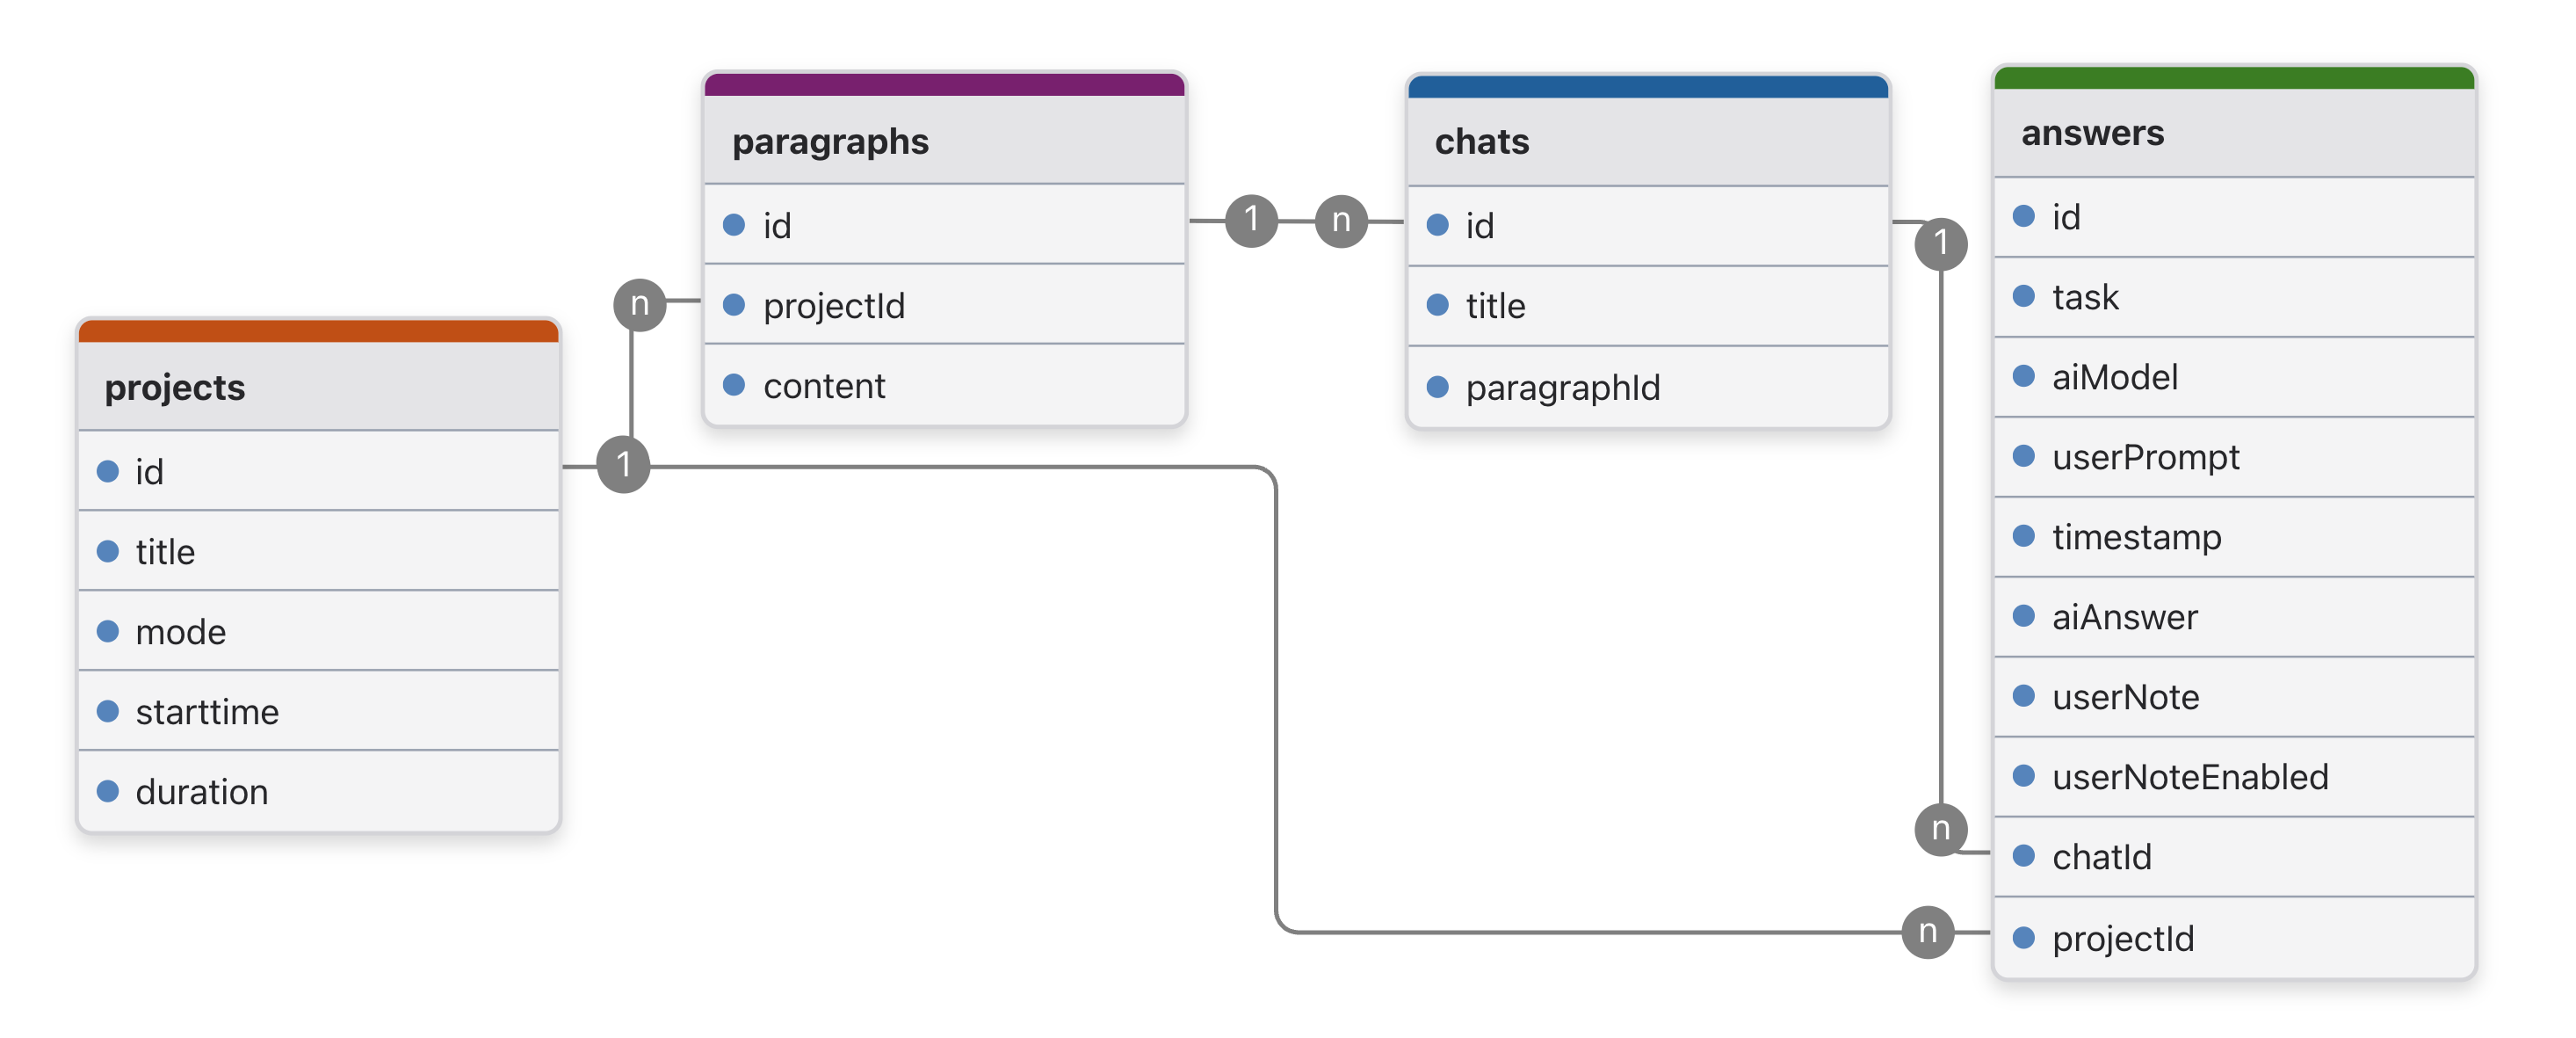
\includegraphics[scale=0.14]{bilder/Datenbank.png}
  \caption{Datenbankschema (Quelle: eigene Darstellung)}
  \label{fig:data}
\end{figure}

Die Datenbank wird in Abb. \ref{fig:data} schematisch dargestellt und umfasst vier miteinander verknüpfte Tabellen. Die erste Tabelle speichert alle projektbezogenen Informationen wie ID, 
Projekttitel und den "`mode"', der den Modus des Projektes angibt. Modus 0 steht für den normalen Modus ohne Einschränkungen, Modus 1 und 2 für den Schülermodus, wobei Modus 2 zusätzlich 
eine Bearbeitungszeit mithilfe von Startzeit und Dauer im Backend vorgibt. Modus 3 (Abgegeben-Modus) ermöglicht nur noch das Lesen des Textes und Generieren des \glslink{glos:ki}{KI}-Nutzungsverzeichnisses, 
eine Bearbeitung ist dann nicht mehr möglich.\\ Jedes Projekt kann mehrere Paragraphen enthalten, die den geschriebenen Text darstellen. Jedem Paragraphen können wiederum mehrere 
\glslink{glos:ki}{KI}-Chats zugeordnet werden, die jeweils einen Titel und mehrere "`Antworten"' ("`answer"') besitzen, welche die eigentlichen Konversationen mit der \glslink{glos:ki}{KI} darstellen. Eine Antwort besteht aus 
der Nutzeranfrage samt allen zu speichernden Daten und einem optionalen Kommentar, der künftigen Anfragen im Chat beigefügt werden kann. Außerdem beinhaltet jede Antwort einen 
Zeitstempel, welcher im \glslink{glos:ki}{KI}-Nutzungsverzeichnis angegeben wird.\\ Zusätzlich gibt es eine direkte Verknüpfung zwischen Projekten und Antworten. Dadurch gehen im 
Schülermodus selbst beim Löschen eines Paragraphen die zugehörigen \glslink{glos:ki}{KI}-Anfragen nicht verloren. So können auch für gelöschte Paragraphen die dazugehörigen \glslink{glos:ki}{KI}-Anfragen 
im Nutzungsverzeichnis dokumentiert und die Nachvollziehbarkeit für Lehrkräfte erhöht werden.



\section{Implementierung der Systemarchitektur und Arbeitsabläufe}
\begin{figure}[h!]
  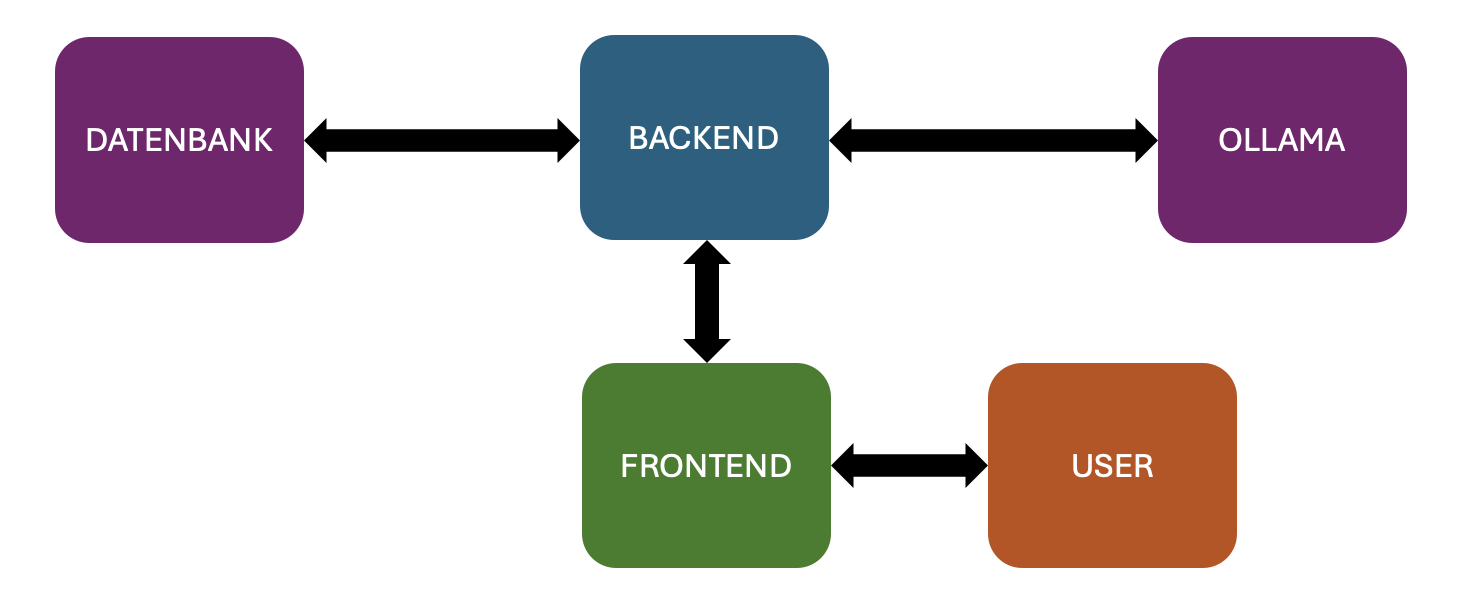
\includegraphics[scale=0.6]{bilder/Architektur.png}
  \caption{Architekturschema (Quelle: eigene Darstellung)}
  \label{fig:architecture}
\end{figure}
Das Backend stellt die nötigen Endpunkte für das Frontend bereit, um Projekte, Paragraphen, Chats und Antworten zu erstellen, zu löschen, abzurufen oder zu bearbeiten, sowie Aufrufe an Ollama 
zu senden (Abb. \ref{fig:architecture}). Das Frontend nutzt diese Endpunkte, um die Funktionalität für den Nutzer bereitzustellen.\\
Bei dem Erstellen eines Projekts im Modus 2 kann eine Bearbeitungszeit festgelegt werden, die über einen Timer angezeigt wird. Läuft die Zeit ab, wird der Modus automatisch auf Modus 3 gesetzt 
und sowohl das \glslink{glos:ki}{KI}-Nutzungsverzeichnis als auch die Text-PDF werden generiert und heruntergeladen. Um zu verhindern, dass Schüler während der Bearbeitung andere Tabs 
oder Programme öffnen, wird die Arbeit beim Verlassen des Browsertabs \cite{react-onblur} oder beim Zurückkehren zum Startbildschirm automatisch abgegeben. Das Projekt 
kann manuell per „Abgeben“-Button abgeschlossen werden.\\
Zum Generieren des \glslink{glos:ki}{KI}-Nutzungsverzeichnisses sendet das Frontend eine Anfrage ans Backend, das ein JSON-Objekt mit den nötigen Informationen zurückliefert. 
Dieses wird im Frontend als PDF formatiert und zum \mbox{Download bereitgestellt.}


\section{Herausforderungen}

Weiterhin wurden Variablen im Frontend bei dem Neuladen der Seite zurückgesetzt und der Timer begann von vorn. Zur Lösung werden Startzeitpunkt und Dauer der Bearbeitungszeit im Backend 
gespeichert.\\ 
Ein weiteres Risiko ist Prompt-Injection, bei dem Schüler versuchen könnten, die vorgesehenen Einschränkungen zu umgehen, indem sie in einigen Feldern oder in Absätzen ganze \gls{glos:prompt}s einfügen.\\ 
Zur Abwehr dieser Versuche gibt es verschiedene Ansätze: Eine Möglichkeit wäre das Filtern der Eingaben, zum Beispiel mittels zwischengeschaltetem \glslink{glos:llm}{LLM} oder das statische Verbieten 
bestimmter Phrasen. Beides wurde verworfen, da dies die Performanz mindert oder den Schreibprozess einschränken könnte. \cite{promptinjection}\\
Das Filtern der Ausgaben ist ungeeignet, da sich neu generierte und umformulierte Texte kaum unterscheiden lassen. Stattdessen wird eine Kombination aus Parametrisierung und \glslink{prompt-engineering}{Prompt-Engineering} 
eingesetzt: Eingabefelder werden meist auf wenige Optionen beschränkt. Wo dies nicht möglich ist, werden die Prompts so gestaltet, dass klar zwischen Nutzereingabe und Systemanweisung \mbox{unterschieden wird.}
\end{document}